\documentclass{nada-ten}
\usepackage[utf8]{inputenc}
\usepackage[swedish,english]{babel}
\usepackage{array}
% \usepackage{qbordermatrix}
\usepackage{graphicx}
\usepackage[dvipsnames]{xcolor}
\graphicspath{{figures/}}
\usepackage{upquote} % this is to make straight apostrophes in verbatim
\usepackage{listings}
\usepackage{mdframed}
\usepackage{tikz}
\usetikzlibrary{calc,fit}
\usepackage{tipa}
\usepackage{amsmath}

\usepackage[
  backend=biber, % for utf8 encoding (dowsn't seem to work)
  %style=numeric
  %natbib=true,
  %abbreviate=true,
  %firstinits=true,
  %maxcitenames=99, % affects citations in the text and labels (problem with \fullcite)
  %mincitenames=2, % affects citations in the text and labels
  %maxbibnames=99  % affects bibliografy only
]{biblatex}

\addbibresource{~/Documents/bib/gs-full.bib}
\addbibresource{~/Documents/bib/IEEEfull.bib}
\addbibresource{~/Documents/bib/gs.bib}

\author{Giampiero Salvi}
\course{DT2119 Speech and Speaker Recognition}
\semester{Spring Term \the\year}
\title{DT2119 Lab2: Hidden Markov Models with Gaussian Emissions}

\begin{document}
\maketitle
%\setlanguage{english}
\section{Objective}
After this exercise you should be able to:
\begin{itemize}
\item implement the algorithms for the evaluation and decoding of Hidden Markov Models (HMMs),
\item use your implementation to perform isolated word recognition,
\item implement the algorithms for training Gaussian Hidden Markov Models (G-HMMs),
\item explain the meaning of the forward, backward and state posterior probabilities evaluated on speech utterances,
%\item \dots {\color{red} FIX ME!}
\end{itemize}
The lab is designed in Python, but the same functions can be obtained in Matlab/Octave.

\section{Task}
The overall task is to implement and test methods for isolated word recognition:
\begin{itemize}
\item combine phonetic HMMs into word HMMs using a lexicon
\item implement the \emph{forward-backward} algorithm,
\item use it compute the log likelihood of spoken utterances given a Gaussian HMM
\item perform isolated word recognition
\item implement the \emph{Viterbi algorithm}, and use it to compute Viterbi path and likelihood
\item compare and comment Viterbi and Forward likelihoods
\item implement the \emph{Baum-Welch algorithm} to update the parameters of the emission probability distributions
\end{itemize}

In order to pass the lab, you will need to follow the steps described in this document, and present your results to a teaching assistant in the designated time slots.

\section{Data and model set}
The speech data used in this lab is similar but not the same as in Lab~1. You can load the  array containing speech utterances with the commands:
\begin{verbatim}
>>> import numpy as np
>>> data = np.load('lab2_data.npz', allow_pickle=True)['data']
\end{verbatim}
The data contains also MFCC features (\texttt{lmfcc} key), but you are welcome to test how the algorithms perform on the MFCCs computed with your own code from Lab~1. Refer to the instructions to Lab~1 for more information about the data structures.

Additionally, the \texttt{lab2\_models\_onespkr.npz} and \texttt{lab2\_models\_all.npz} files contain the parameters of the models you are going to use to test your functions and the \texttt{lab2\_example.npz} file contains an example that can be used for debugging.

\subsection{The phonetic models}
The models you will use in the exercise were trained on the TIDIGITS database with 13 MFCC feature vectors computed as in Lab~1.
The lab package contains two versions of the models that you will have to compare:
\begin{itemize}
\item \texttt{lab2\_models\_all.npz} was trained on the full training set,
\item \texttt{lab2\_models\_onespkr.npz} was trained on a single speaker, that happens to be female.
\end{itemize}

Load one of the model files with:
\begin{verbatim}
>>> phoneHMMs = np.load('lab2_models_onespkr.npz', allow_pickle=True)['phoneHMMs'].item()
\end{verbatim}
or
\begin{verbatim}
>>> phoneHMMs = np.load('lab2_models_all.npz', allow_pickle=True)['phoneHMMs'].item()
\end{verbatim}
The resulting variable \texttt{phoneHMMs} is a dictionary with 21 keys each corresponding to a phonetic model. You can list the model names with:
\begin{verbatim}
>>> list(sorted(phoneHMMs.keys()))
['ah', 'ao', 'ay', 'eh', 'ey', 'f', 'ih', 'iy', 'k', 'n', 'ow', 'r', 's',
 'sil', 'sp', 't', 'th', 'uw', 'v', 'w', 'z']
\end{verbatim}

Special cases are \texttt{sil} and \texttt{sp} that model silence and short pauses.
For this exercise you can ignore the \texttt{sp} model, that will become important only in Lab~3.
Note that the list is a subset of the phonemes used in the English language limited to the pronunciation of the 11 digits.

Each model is an HMM with a single Gaussian emission probability distribution per state and diagonal covariance matrices stored as vectors.

Each model contains the following keys:
\begin{verbatim}
>>> phoneHMMs['ah'].keys()
['name', 'startprob', 'transmat', 'means', 'covars']
\end{verbatim}

%Both the HMMs and the GMMs were trained on the same data (different from the data in the \texttt{tidigits} array) and were initialized the same way. Both use diagonal covariance matrices for the Gaussian distributions. The size of the model (number of states in HMM and number of Gaussians in GMM) depends on the digit and was obtained using three states for each phoneme in \verb|models[i]['pron']| plus three states for the initial and final silence in the utterance. For example, the digit \verb|'6'| is pronounced as \verb|['s', 'ih', 'k', 's']| and will therefore have $(4+2)\times 3 = 18$ states.

\begin{center}
\begin{tabular}{llp{0.5\textwidth}}
  key & symbol & description \\
  \hline
  \texttt{name} & & phonetic symbol, \texttt{sil} or \texttt{sp} \\
  \texttt{startprob} & $\pi_i = P(z_0=s_i)$ & probability to start in state $i$ \\
  \texttt{transmat}: & $a_{ij} = P(z_n=s_j|z_{n-1}=s_i)$ & transition probability from state $i$ to $j$ \\
  \texttt{means}: & $\mu_{id}$ & array of mean vectors (rows correspond to different states) \\
  \texttt{covars}: & $\sigma^2_{id}$ & array of variance vectors (rows correspond to different states) \\
  \hline
\end{tabular}
\end{center}

If you ignore the \texttt{sp} model, all models have three emitting states.
Consequently, the \texttt{means} and \texttt{covars} arrays will be both $3\times 13$ in size.
Note, however, that both the \texttt{startprob} and \texttt{transmat} arrays have sizes corresponding to four states (\texttt{startprob} is length $4$ and \texttt{transmat} is $4 \times 4$).
The reason for this is that we will concatenate these models to form word models, and we therefore want to be able to express the probability $a_{i3}$ to leave the model from state $s_i$.

In the left-to-right models you will use in this exercise the model can only be left from the last (third) emitting state in each phonetic model $s_2$ (with probability $a_{23}$).
This is illustrated in the following figure and will be clearer in Section~\ref{sec:word_models}.
\begin{center}
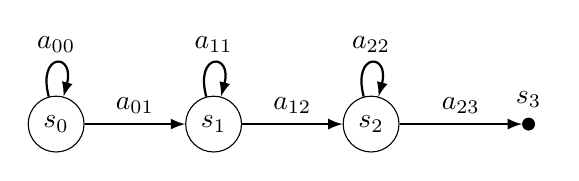
\begin{tikzpicture}
  \tikzstyle{directed}=[-latex, thick, color=red]
  \foreach \x in {0,...,2} {
    \node[circle,draw,minimum size=4mm] (s\x) at ({\x*2},0) {$s_\x$};
  }
  \node[circle,draw,fill, inner sep=0pt,minimum size=1.5mm, label={$s_3$}] (s3) at ({3*2},0) {};
  \foreach \x/\y in {0/1,1/2,2/3} {
    \path[directed,black] (s\x) edge node[above] {$a_{\x\y}$} (s\y);
    \draw[directed,black] (s\x) to[loop above] node[above] {$a_{\x\x}$} (s\x);
  }
  % \draw[directed,black] (s6) to[loop left] (s6);
\end{tikzpicture}
\end{center}

Note that the last state $s_3$ is non-emitting, meaning that it does not have any state to output probability distribution associated with it.

% Check the transition matrix and the start probability for the HMM models. What can you say about their topology (transition structure)?

% \subsection{The models}
% Load the model file with:
% \begin{verbatim}
% models = np.load('lab2_models.npz')['models']
% \end{verbatim}

% The \texttt{models} array has length 11 each element corresponding to one of the following digits: \verb|['o','z','1','2','3','4','5','6','7','8','9']|. Each element contains the following keys:
% \begin{verbatim}
% models[0].keys()
% ['digit', 'pron', 'hmm', 'gmm']
% \end{verbatim}

% \begin{center}
% \begin{tabular}{lp{0.8\textwidth}}
%   key & description \\
%   \hline
%   \texttt{digit}: & the digit the model refers to \\
%   \texttt{pron}: & pronunciation of the digit in terms of phonemes (not needed in this exercise) \\
%   \texttt{hmm}: & model parameters of a Gaussian HMM trained with Baum-Welch \\
%   \texttt{gmm}: & model parameters of a GMM trained with EM \\
%   \hline
% \end{tabular}
% \end{center}

% Both the HMMs and the GMMs were trained on the same data (different from the data in the \texttt{tidigits} array) and were initialized the same way. Both use diagonal covariance matrices for the Gaussian distributions. The size of the model (number of states in HMM and number of Gaussians in GMM) depends on the digit and was obtained using three states for each phoneme in \verb|models[i]['pron']| plus three states for the initial and final silence in the utterance. For example, the digit \verb|'6'| is pronounced as \verb|['s', 'ih', 'k', 's']| and will therefore have $(4+2)\times 3 = 18$ states.

% The HMM model contains the following fields:

% \begin{verbatim}
% models[0]['hmm'].keys()
% ['startprob', 'transmat', 'means', 'covars']
% \end{verbatim}

% \begin{center}
% \begin{tabular}{llp{0.5\textwidth}}
%   key & symbol & description \\
%   \hline
%   \texttt{startprob} & $\pi_i = P(z_0=s_i)$ & probability to start in state $i$ \\
%   \texttt{transmat}: & $a_{ij} = P(z_n=s_j|z_{n-1}=s_i)$ & transition probability from state $i$ to $j$ \\
%   \texttt{means}: & $\mu_{id}$ & array of mean vectors (rows correspond to different states) \\
%   \texttt{covars}: & $\sigma^2_{id}$ & array of variance vectors (rows correspond to different states) \\
%   \hline
% \end{tabular}
% \end{center}

% The GMM models contain the following fields:

% \begin{verbatim}
% models[0]['gmm'].keys()
% ['weights', 'means', 'covars']
% \end{verbatim}

% \begin{center}
% \begin{tabular}{lll}
%   key & symbol & description \\
%   \hline
%   \texttt{weights}: & $w_i$ & weight of each Gaussian in the mixture \\
%   \texttt{means}: & $\mu_{id}$ & array of mean vectors (rows correspond to different Gaussians) \\
%   \texttt{covars}: & $\sigma^2_{id}$ & array of variance vectors (rows correspond to different Gaussians) \\
%   \hline
% \end{tabular}
% \end{center}

% Check the transition matrix and the start probability for the HMM models. What can you say about their topology (transition structure)?
\subsection{Pronunciation dictionary and utterance models}
\label{sec:word_models}
The mapping between digits (words) and phonetic models can be obtained with the pronunciation dictionary that you can find in \texttt{prondict.py}, and that looks like this:
\begin{verbatim}
prondict = {}
prondict['o'] = ['ow']
prondict['z'] = ['z', 'iy', 'r', 'ow']
prondict['1'] = ['w', 'ah', 'n']
...
\end{verbatim}
% prondict['2'] = ['t', 'uw']
% prondict['3'] = ['th', 'r', 'iy']
% prondict['4'] = ['f', 'ao', 'r']
% prondict['5'] = ['f', 'ay', 'v']
% prondict['6'] = ['s', 'ih', 'k', 's']
% prondict['7'] = ['s', 'eh', 'v', 'ah', 'n']
% prondict['8'] = ['ey', 't']
% prondict['9'] = ['n', 'ay', 'n']

Because we are working with recordings of isolated digits, a model of each utterance should also contain initial and final silence:
\begin{verbatim}
>>> isolated = {}
>>> for digit in prondict.keys():
>>>    isolated[digit] = ['sil'] + prondict[digit] + ['sil']
\end{verbatim}

\section{Concatenating HMMs}
Write the \texttt{concatTwoHMMs} function in \texttt{lab2\_proto.py} that takes two HMMs in input and returns an HMM that is the concatenation of the two.
Refer to the included \texttt{concatenating\_hmms.pdf} document for a detailed description on how to combine the state priors, transition matrices and emission probability distributions from each model. 

Then use the already defined \texttt{concatHMMs} in \texttt{lab2\_proto.py} to concatenate any number of HMMs, given a set of HMM models and a list of model names. For example:

\begin{verbatim}
>>> wordHMMs = {}
>>> wordHMMs['o'] = concatHMMs(phoneHMMs, isolated['o'])
\end{verbatim}

In this case, \verb|isolated['o']=['sil', 'ow', 'sil]|, and the resulting word model will be a concatenation of three models with three emitting states each as illustrated below:

\newcommand{\hmm}[1]{
\begin{tikzpicture}
  \tikzstyle{directed}=[-latex, thick, color=red]
  \foreach \x in {0,...,2} {
    \node[circle,draw,fill=#1,inner sep=1pt,minimum size=4mm] (s\x) at (\x,0) {$s_\x$};
  }
  \node[circle,draw,fill, inner sep=0pt,minimum size=1.5mm,label={$s_3$}] (s3) at (3,0) {};
  \foreach \x/\y in {0/1,1/2,2/3} {
    \draw[directed,black] (s\x) -- (s\y);
    \draw[directed,black] (s\x) to[loop above] (s\x);
  }
  % \draw[directed,black] (s6) to[loop left] (s6);
\end{tikzpicture}
}

\begin{center}
\hmm{red!30} \hspace{1cm} \hmm{blue!20} \hspace{1cm} \hmm{green!60}

$\Huge\Downarrow$

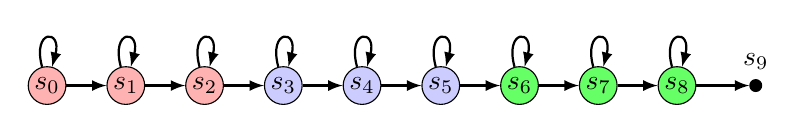
\begin{tikzpicture}
  \tikzstyle{directed}=[-latex, thick, color=red]
  \foreach \x in {0,...,2} {
    \node[circle,draw,fill=red!30,inner sep=1pt,minimum size=4mm] (s\x) at (\x,0) {$s_\x$};
  }
  \foreach \x in {3,...,5} {
    \node[circle,draw,fill=blue!20,inner sep=1pt,minimum size=4mm] (s\x) at (\x,0) {$s_\x$};
  }
  \foreach \x in {6,...,8} {
    \node[circle,draw,fill=green!60,inner sep=1pt,minimum size=4mm] (s\x) at (\x,0) {$s_\x$};
  }
  \node[circle,draw,fill, inner sep=0pt,minimum size=1.5mm,label={$s_9$}] (s9) at (9,0) {};
  \foreach \x/\y in {0/1,1/2,2/3,3/4,4/5,5/6,6/7,7/8,8/9} {
    \draw[directed,black] (s\x) -- (s\y);
    \draw[directed,black] (s\x) to[loop above] (s\x);
  }
  % \draw[directed,black] (s6) to[loop left] (s6);
\end{tikzpicture}
\end{center}

Remember that each model in \texttt{phoneHMMs} has an extra state to simplify the concatenation.
All the extra states but the last are dropped when doing the concatenation.

\subsection{The example}
Load the example file with:
\begin{verbatim}
example = np.load('lab2_example.npz', allow_pickle=True)['example'].item()
\end{verbatim}
This is a dictionary containing all the fields as in the \texttt{data} array, plus the following additional fields:
\begin{verbatim}
list(example.keys())
[..., 'obsloglik', 'logalpha', 'loglik', 'vloglik', 'loggamma', 'logxi']
\end{verbatim}
%'hmm_logbeta',

Here is a description of each field. You will see how to use this information in the reminder of these instructions. All the probabilities described below were obtained using the HMM model \verb|wordHMMs['o']| (that is, the models for digit \verb|'o'| with phonetic models taken from \texttt{lab2\_models\_onespkr.npz}) on the sequence of MFCC vectors in \verb|example['lmfcc']|. Also with \texttt{n\_states} we intend the number of emitting states in the model, that is the length of \texttt{startprob} minus one:

\begin{center}
\begin{tabular}{lclp{0.5\textwidth}}
  key & idxs & symbol & description \\
  \hline
  %\texttt{gmm\_obsloglik} & \texttt{[i,j]} & $\log\phi_j(x_i)$ & observation log likelihood for each Gaussian in \texttt{models[0][gmm]}, shape: (n\_timesteps, n\_gaussians) \\
  %\texttt{gmm\_loglik} & - & $\log P(X|\theta_{\mbox{\tiny GMM}})$ & log likelihood of the observations sequence $X$ given the full GMM model, scalar \\
  \texttt{obsloglik} & \texttt{[i,j]} & $\log\phi_j(x_i)$ & observation log likelihood for each Gaussian in \verb|wordHMMs['o']|, shape: \texttt{(n\_timesteps, n\_states)} \\
  \texttt{logalpha} & \texttt{[i,j]} & $\log\alpha_i(j)$ & alpha log probabilities, see definition later, shape: \texttt{(n\_timesteps, n\_states)} \\
  \texttt{logbeta} & \texttt{[i,j]} & $\log\beta_i(j)$ & beta log probabilities, see definition later, shape: \texttt{(n\_timesteps, n\_states)} \\
  \texttt{loglik} & - & $\log P(X|\theta_{\mbox{\tiny HMM}})$ & log likelihood of the observations sequence $X$ given the HMM model, scalar \\
  \texttt{vloglik} & - & $\log P(X,S_{\mbox{opt}}|\theta_{\mbox{\tiny HMM}})$ & Viterbi log likelihood of the observations sequence $X$ and the best path given the HMM model, scalar \\
  \texttt{loggamma} & \texttt{[i,j]} & $\log \gamma_i(j)$ & gamma log probabilities, see definition later, shape: \texttt{(n\_timesteps, n\_states)} \\
  \texttt{logxi} & \texttt{[i,j]} & $\log \xi_i(j)$ & xi log probabilities, see definition later, shape: \texttt{(n\_timesteps, n\_states)} \\
  \hline
\end{tabular}
\end{center}
\vspace{2mm}

Figure~\ref{fig:example} shows some of the relevant fields in \texttt{example}.

\begin{figure}
  \centering
  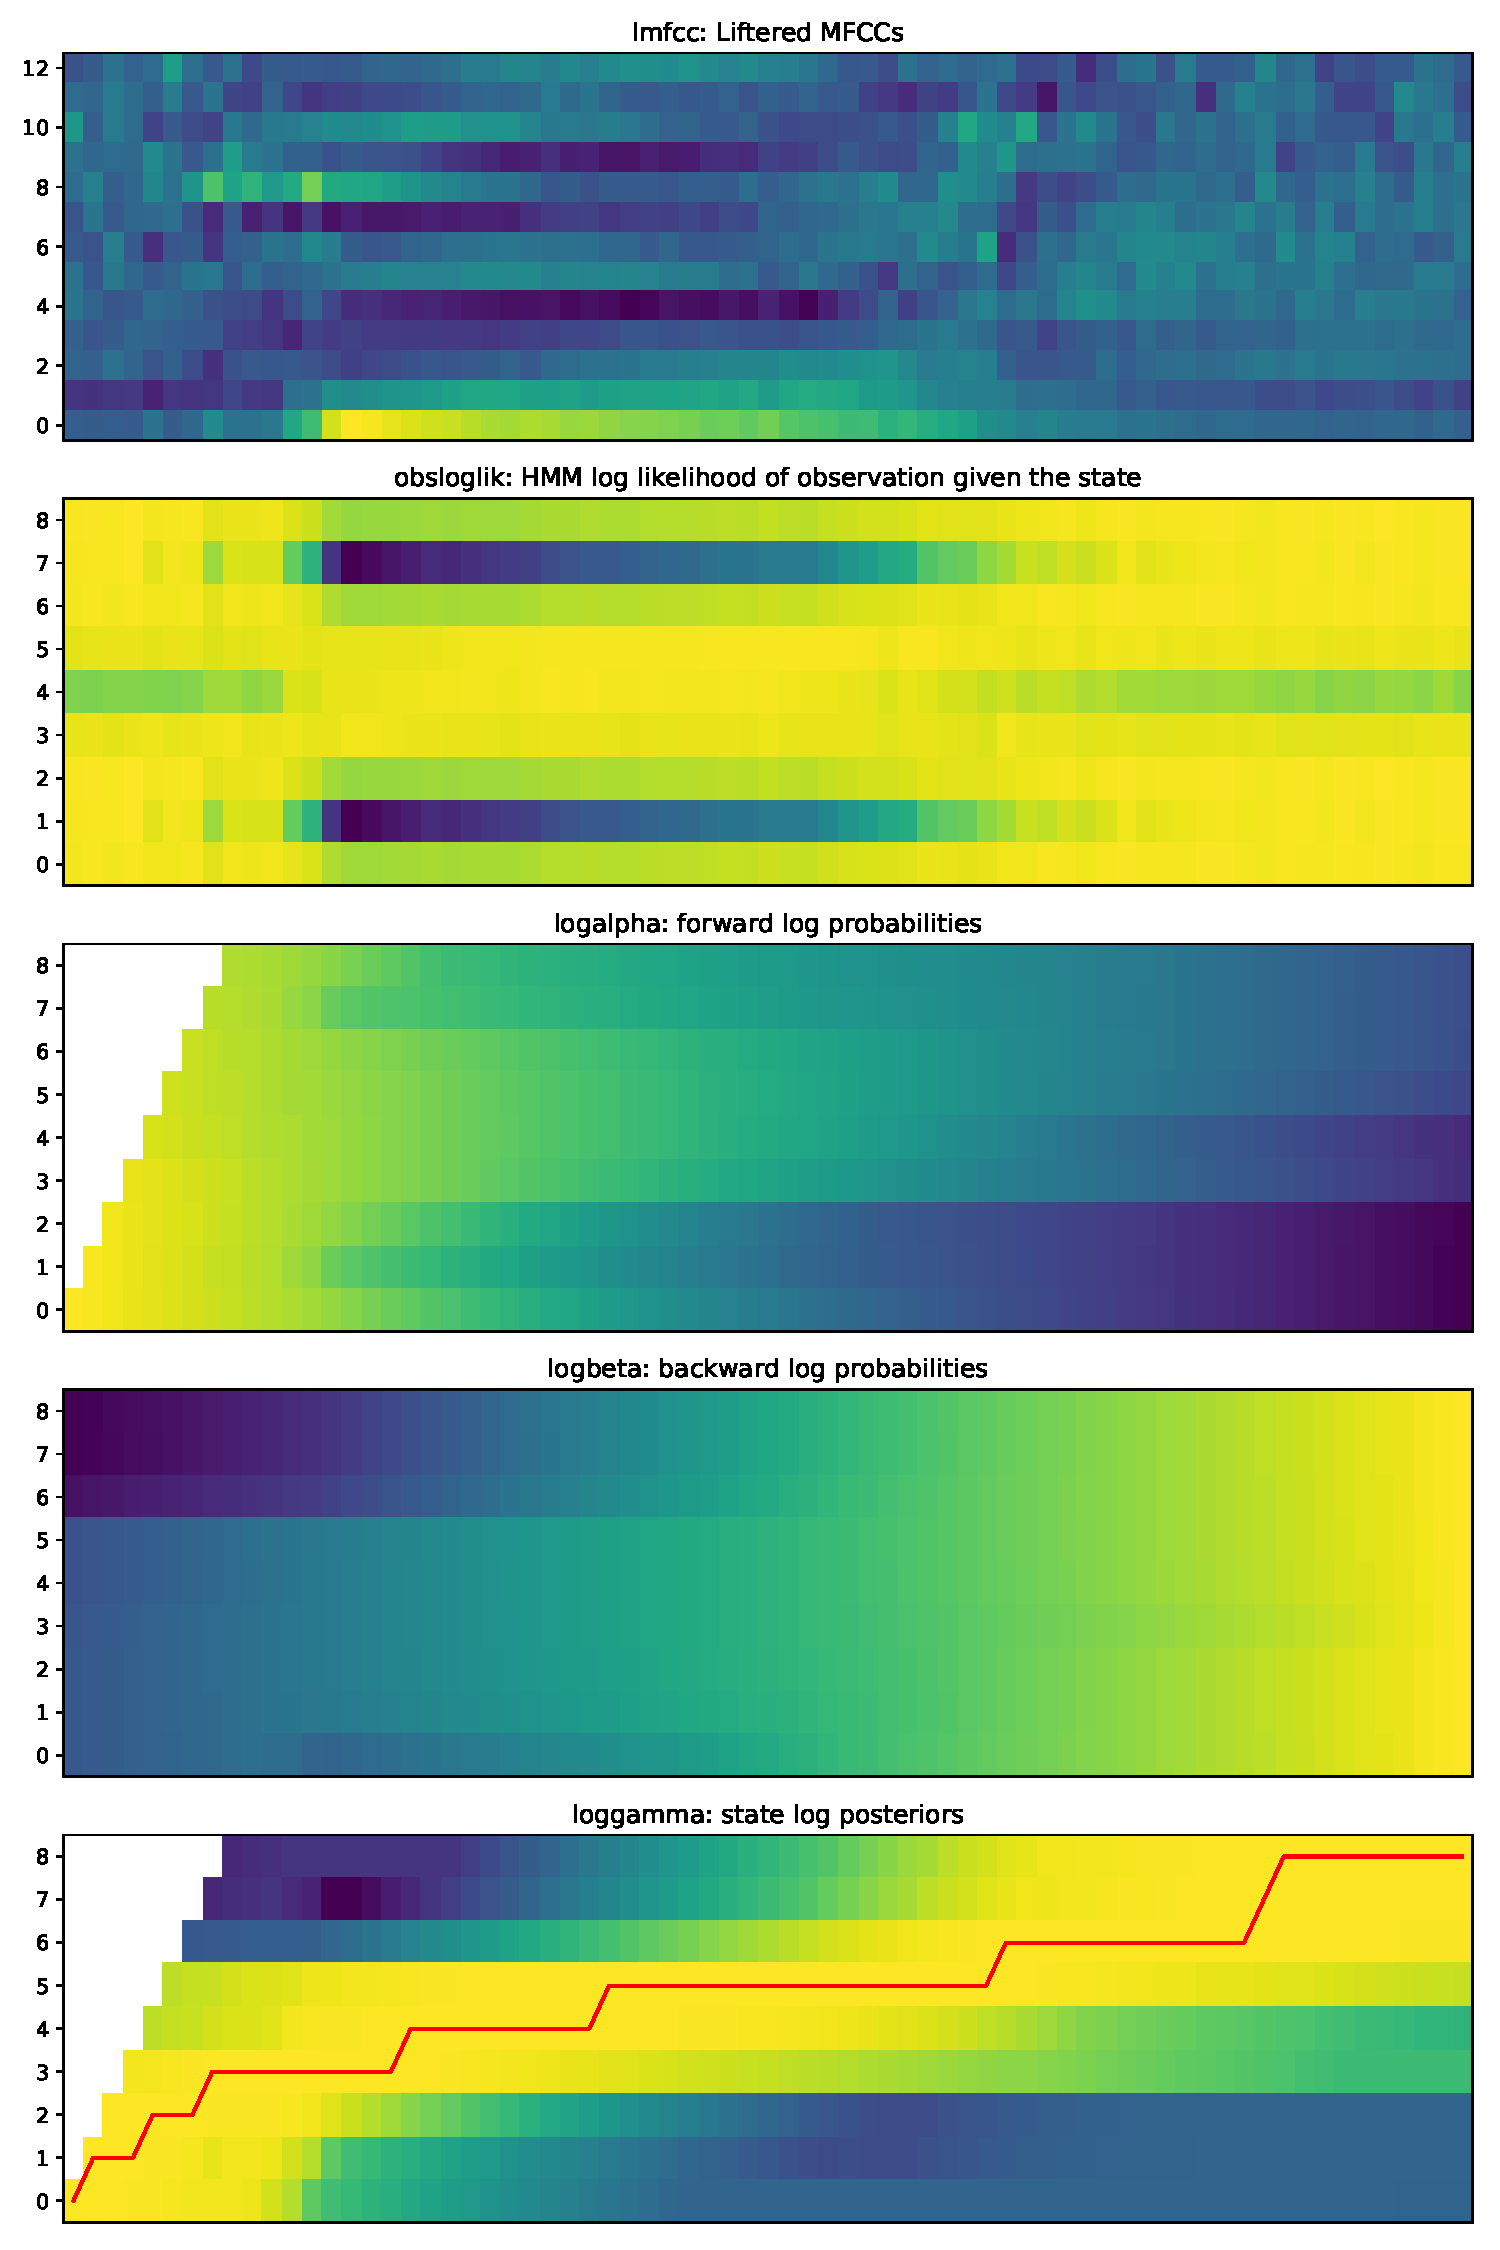
\includegraphics[height=0.9\textheight]{Probabilities_step_by_step}
  \caption{Step-by-step probability calculations for the utterance in the example. The utterance contains the digit ``oh'' spoken by a female speaker. The model parameters are obtained by concatenating the HMM models for \texttt{sil}, \texttt{ow} and \texttt{sil}.}
  \label{fig:example}
\end{figure}

% \section{Old concatHMMs text}
% The following figure tries to explain how the transition matrices are combined to form the resulting transition matrix.
% \begin{center}
% \begin{tikzpicture}
%   \foreach \x in {0,...,9} {
%     \foreach \y in {0,...,9} {
%       %\node[circle,draw,fill, inner sep=0pt,minimum size=1.5mm] (a\x\y) at (\x,-\y) {};
%       \node (a\x\y) at ({\y*0.7},{-\x*0.7}) {$a_{\x\y}$};
%     }
%   }
%   %\node[draw, inner sep=0mm, fit=(a00) (a33)] {};
%   %\node[draw, inner sep=0mm, fit=(a33) (a66)] {};
%   %\node[draw, inner sep=0mm, fit=(a66) (a99)] {};
%   \node[draw, inner sep=0mm, fill=red, opacity=0.2, fit=(a00) (a33)] {};
%   \node[draw, inner sep=0mm, fill=blue, opacity=0.2, fit=(a33) (a66)] {};
%   \node[draw, inner sep=0mm, fill=green, opacity=0.2, fit=(a66) (a99)] {};
% \end{tikzpicture}
% \end{center}

% Note that this way of concatenation is valid under the following assumptions for each of the original models:
% \begin{enumerate}
% \item the a priori probability of the states $\pi_i$ is non-zero only for the first state
% \item there is only one transition into the last non-emitting state, and it comes from the second last state.
% \end{enumerate}
% To be precise, we should remove the last row from the transition matrix of the red and blue models. However, in each original transition matrix, because of the second assumption above, the last row is $ [0.0, 0.0, 0.0, 1.0] $. If we copy the values in into the new transition matrix in the natural order (red, blue, green), the first element of new transition matrix will overwrite the last of the previous one, and we would obtain the same affect. The last row of the combined transition matrix will also be all zeros but one ($a_{99}$ in this case).

% The \texttt{means} and \texttt{covars} matrices are simply concatenated because they are only defined for the emitting states in the original models.
\clearpage
\section{HMM Likelihood and Recognition}
\subsection{Gaussian emission probabilities}
The function \texttt{log\_multivariate\_normal\_density\_diag()} from \texttt{lab2\_tools.py} can be used to compute
$$ \mbox{obsloglik}[i,j] = \log \phi_j(x_i) = \log N(x_i, \mu_j, \Sigma_j) = \log P(x_i|\mu_j,\Sigma_j),$$
that is the log likelihood for each observation $x_i$ and each term in a multivariate Gaussian density function with means $\mu_j$ and diagonal covariance matrices $\Sigma_j$. In the case of Gaussian HMMs, $\phi_j$ corresponds to the emission probability model for a single state $j$. %In case of a GMM, $\phi_j$ corresponds to a single Gaussian in the model, without considering the weights.

Verify that you get the same results as in \verb|example['obsloglik']| %and \\\verb|example['gmm_obsloglik']|
when you apply the \texttt{log\_multivariate\_normal\_density\_diag} function to the \verb|example['lmfcc']| data using the Gaussian distributions defined by the \verb|wordHMMs['o']| that you have created with your \texttt{concatHMMs} function. Note that in these cases we are not using the time dependency structure of the HMM, but only the Gaussian distributions.

Plot the log likelihood for Gaussians from HMMs models corresponding to the same digit on a test utterance of your choice. What can you say about the figure? Which Gaussian components give the high likelihood in which time steps? Why? Remember that each utterance starts and ends with silence.

% \section{GMM Likelihood and Recognition}
% Based on the output of the function in the previous section, write the \texttt{gmmloglik} function (\texttt{lab2_proto.py}) that computes the log likelihood of an observation sequence $X=\{x_0, \dots, x_{N-1}\}$ given the full GMM model, that is, given the weights of each Gaussian density in the GMM model. Remember that the assumption in the GMM model is that the $x_n$ vectors are independent for each $n=[0,N)$\footnote{We are using the convention to express intervals with square brackets ``$[$'' if the extreme is included and parentheses ``$)$'' if it is excluded. This corresponds to the \texttt{range} function in Python that includes the start value but not the end value.}. Whenever there is an expression involving the log of a sum of exponents ($\log\sum\exp(.)$), make use of the \texttt{logsumexp} function from \texttt{lab2_tools.py}.

% The output of the \texttt{gmmloglik} function, using the model parameters in \verb|models[0]['gmm']| and the observation sequence from \verb|example['lmfcc']|, should correspond to \verb|example['gmm_loglik']|.

% Use this function to score each of the 44 utterances in the \texttt{tidigits} array with each of the 11 GMM models in \verb|models[i]['gmm']|. If we select for each utterance the model with the highest log likelihood, how many digits are misrecognized?

\subsection{Forward Algorithm}
Write the function \texttt{forward} following the prototypes in \texttt{lab2\_proto.py}. The function should take as input a lattice of emission probabilities as in the previous section, that is an array containing:
\begin{eqnarray*}
 \mbox{obsloglik}[i,j] &=& \log \phi_j(x_i)
\end{eqnarray*}
and the model parameters $a_{ij}$ and $\pi_i$. When you compute the log of $a_{ij}$ and $\pi_i$, some of the values will become negative infinity ($\log(0)$). This should not be a problem, because all the formulas should remain consistent and you should only get a warning from \texttt{numpy}\footnote{If you do not want to get the warnings, you can add: \texttt{import warnings} and \texttt{warnings.filterwarnings("ignore", category=RuntimeWarning)} at the beginning. An alternative would be to use the function \texttt{numpy.ma.log()} which will mask $\log(0)$ elements, but at the time of writing I could not get this to work properly, so I do not recommend it at this point.}.

The output is the array:
\begin{eqnarray*}
  \mbox{logalpha}[i,j] &=& \log\alpha_i(j)
\end{eqnarray*}
where $i$ corresponds to time steps and $j$ corresponds to states in the model.
%You can find the recursion formulae for the forward probabilities in \emph{log domain} in the slides (you might have to adjust the indices to follow Python and C conventions).

%The recursion formulae for the forward probabilities in \emph{log domain} are given here, where we have used Python convention with array indices going from 0 to len-1:
%\begin{eqnarray*}
%  \log\alpha_0(j) &=& \log\pi_j + \log\phi_j(x_0) \\
%  \log\alpha_n(j) &=& \log\left(\sum_{i=0}^{M-1} \exp\Big(\log\alpha_{n-1}(i) + \log a_{ij}\Big)\right) + \log\phi_j(x_n)
%\end{eqnarray*}

Remember that the forward probability is defined as:
\begin{eqnarray}
  \alpha_n(j) &=& P(x_0, \dots, x_n, z_n=s_j|\theta), \label{eqn:forward}
\end{eqnarray}
where $\theta = \{\Pi, A, \Phi\}$ are the model parameters. 
There is a recursion formula (see Appendix~\ref{sec:recursions}) to obtain $\alpha_n(j)$ from $\alpha_{n-1}(i)$ for all the previous states.
In the recursion formulae for the forward (and backward) probabilities there is an expression involving the log of a sum of exponents ($\log\sum\exp(.)$). Make use of the \texttt{logsumexp} function from \texttt{lab2\_tools.py} to calculate those cases.

Apply your function to the \verb|example['obsloglik']| utterance using the model parameters in your \verb|wordHMMs['o']| model and verify that you obtain the same $\log\alpha$ array as in \verb|example['logalpha']|.

%The definitions of $\alpha_n(j)$ in terms of probabilities of events are defined below ():
%\begin{eqnarray*}
%  \alpha_n(j) &=& P(x_0, \dots, x_n, z_n=s_j|\theta)
%\end{eqnarray*}
Remembering the definition of $\alpha$ in Eqn.~\ref{eqn:forward}, derive the formula to compute the likelihood $P(X|\theta)$ of the whole sequence $X = \{x_0, \dots, x_{N-1}\}$, given the model parameters $\theta$ in terms of $\alpha_n(j)$.

\begin{mdframed}
\textbf{Hint:} if the events $B_j, j\in[0, M)$ form a disjoint partition of the sure event, that is:
\begin{eqnarray*}
  P(B_i,B_j)&=&0,\ \ \  \forall i,j,\ \ i\neq j,\ \ \mbox{and} \\
  \sum_{j=0}^{M-1}P(B_j)&=&1,
\end{eqnarray*}
then it is true that $P(A) = \sum_{j=0}^{M-1} P(A,B_j)$, that is, we can \emph{marginalize out} the variable $B_j$.
\end{mdframed}

% is as follows:
%\begin{eqnarray}
% P(X|\theta) = \sum_{j=0}^{M-1} \alpha_{N-1}(j),
%\end{eqnarray}
%that is, we need to sum the alphas over all the states in the model at the last time step. In log domain, the same formula will be:
%\begin{eqnarray}
% \log P(X|\theta) = \log\sum_{j=0}^{M-1}\exp(\log\alpha_{N-1}(j)).
% \label{eqn:alphatotal}
%\end{eqnarray}

Convert the formula you have derived into log domain.
Verify that the log likelihood obtained this way using the model parameters in \verb|wordHMMs['o']| and the observation sequence in \verb|example['lmfcc']| is the same as \verb|example['loglik']|.

%Eqn.~\ref{eqn:alphatotal}, 
Using your formula, score all the 44 utterances in the \texttt{data} array with each of the 11 HMM models in \texttt{wordHMMs}. Do you see any mistakes if you take the maximum likelihood model as winner? Compare the results obtained from the models trained on a single speaker or all the training speakers.

% Compare these results with the GMM results obtained in the previous session.
%Repeat the recognition using the Gaussian distributions in the HMM models as if they were a GMM model with equal weights for each Gaussian. What can you say about the results you obtain this way? Can you say something about the influence of the HMM transition model in this particular task?

%Plot the $\alpha$ lattice (that is the array of $\alpha$s for each time step and state). What can you say about the influence of the HMM topology on the first time steps? How about the last ones?

\subsection{Viterbi Approximation}
Here you will compute the log likelihood of the observation $X$ given a HMM model and the best sequence of states. This is called the Viterbi approximation. Implement the function \texttt{viterbi} in \texttt{lab2\_proto.py}. 

In order to recover the best path, you will also need an array storing the best previous path for each time step and state (this needs to be defined only for $n\in[1,N)$, that is not for the first time step):

\begin{eqnarray*}
  B_n(j) &=& \arg\max_{i=0}^{M-1} \Big(\log V_{n-1}(i) + \log a_{ij}\Big)
\end{eqnarray*}

Consult the course book \cite{gs:HuangEtAl2001Book}, Section~8.2.3, to see the details of the implementation (note that the book uses indices from 1, instead of 0).

Compute the Viterbi log likelihood for \verb|wordHMMs['o']| and \verb|example['lmfcc']|, and verify that you obtain the same result as in \verb|example['vloglik']|.

Plot the alpha array that you obtained in the previous Section and overlay the best path obtained by Viterbi decoding. Can you explain the reason why the path looks this way?

Using the Viterbi algorithm, score all the 44 utterances in the \texttt{data} with each of the 11 HMM models in \texttt{wordHMMs}. How many mistakes can you count if you take as winner the model with the maximum viterbi score? Are these the same mistakes obtained in previous section? Can you say something about the complexity of the viterbi scoring compared to the forward scoring (for example by measuring the CPU usage?)

\subsection{Backward Algorithm}
Write the function \texttt{backward} following the prototypes in \texttt{lab2\_proto.py}. Similarly to the function \texttt{forward} in the previous section, the function should take as input a lattice of emission probabilities as in the previous section, that is an array containing:
$$ \mbox{obsloglik}[i,j] = \log \phi_j(x_i) $$

The output is the array:
\begin{eqnarray*}
  \mbox{logbeta}[i,j] &=& \log\beta_i(j),
\end{eqnarray*}
where $i$ corresponds to time steps and $j$ corresponds to states in the model. See Appendix~\ref{sec:recursions} for the recursion formulae.

In all the cases where there is an expression involving the log of a sum of exponents ($\log\sum\exp(.)$), make use of the \texttt{logsumexp} function in \texttt{lab2\_tools.py}.

Apply your function to the \verb|example['lmfcc']| utterance using the model parameters in \verb|wordHMMs['o']| and verify that you obtain the $\log\beta$ arrays as in \verb|example['logbeta']|.

The definitions of $\beta_n(j)$ in terms of probabilities of events are defined below (where $\theta = \{\Pi, A, \Phi\}$ are the model parameters):
\begin{eqnarray*}
  \beta_n(i) &=& P(x_{n+1}, \dots, x_{N-1}|z_n=s_i, \theta)
\end{eqnarray*}

\begin{mdframed}
Optional: Derive the formula that computes $P(X|\theta)$ using the betas $\beta_n(i)$ instead of the alphas.
\begin{description}
 \item[Hint 1:] only the $\beta_0(i)$ are needed for the calculation.
 \item[Hint 2:] note that the definition of $\alpha_n(j)$ is a \emph{joint} probability of observations \emph{and} state at time step $n$ whereas $\beta_n(i)$ is a \emph{conditional} probability of the observations \emph{given} the state at time step $n$.
 \item[Hint 3:] the calculation will not only involve the betas, but also some of the observation likelihoods $\phi_j(x_n)$ and some of the model parameters, $\pi_i$ or $a_{ij}$.
\end{description}

Verify that also this method gives you the same log likelihood and that they both are equal to \verb|example['loglik']|.
\end{mdframed}

% \section{Optional: Training}
% Here you will update the model parameters in \verb|models[0]['hmm']| by performing one iteration of the Baum-Welch algorithm with the observation sequence defined in \verb|example['mfcc']|. You will update only the transition probability \verb|models[0]['hmm']['transmat']|, that is $a_{ij} = P(z_n=s_j|z_{n-1}=s_i)$.

% In order to update the transition probabilities, you need to estimate and maximize the probability  $P(z_{n-1}=s_i, z_n=s_j|X, \theta_c)$ of making a particular transition from state $s_i$ to state $s_j$ at the time $n$, with the same conditioned to the observation sequence and the current model parameters.

% Given that you can compute $P(X|\theta_c)$

% You can express the two above probabilities in terms of $\alpha$ and $\beta$ in the following way:
% \begin{eqnarray*}
%   P(z_n=s_j|X, \theta_c) &=& \frac{\alpha_n(j)\beta_n(j)}{P(X|\theta_c)} \\
%   P(z_{n-1}=s_i, z_n=s_j|X, \theta_c) &=& \frac{\alpha_{n-1}(i)a_{ij}\phi_j(x_n)\beta_n(j)}{P(X|\theta_c)},
% \end{eqnarray*}
% % \begin{eqnarray*}
% %   P(z_n=s_j|X, \theta_c) &=& \frac{\alpha_n(j)\beta_n(j)}{\sum_{i=0}^{M-1}\alpha_n(i)} \\
% %   P(z_{n-1}=s_i, z_n=s_j|X, \theta_c) &=& \frac{\alpha_{n-1}(i)a_{ij}\phi_j(x_n)\beta_n(j)}{\sum_{i=0}^{M-1}\alpha_n(i)},
% % \end{eqnarray*}
% % or in log domain:
% % \begin{eqnarray*}
% %   P(z_n=s_j|X, \theta_c) &=& \frac{\alpha_n(j)\beta_n(j)}{\sum_{i=0}^{M-1}\alpha_n(i)} \\
% %   P(z_{n-1}=s_i, z_n=s_j|X, \theta_c) &=& \frac{\alpha_{n-1}(i)a_{ij}\phi_j(x_n)\beta_n(j)}{\sum_{i=0}^{M-1}\alpha_n(i)},
% % \end{eqnarray*}

\section{HMM Retraining (emission probability distributions)}

\subsection{State posterior probabilities}
Implement the \texttt{statePosteriors} function in \texttt{lab2\_proto.py} that calculates the state posteriors $\gamma_n(i) = P(z_n=s_i|X,\theta)$ given the observation sequence, also called gamma probabilities. See Appendix~\ref{sec:recursions} for the formulas in log domain. Calculate the state posteriors for the utterance in the example. Verify that for each time step the state posteriors sum to one (in linear domain).

Consider the emission probabilities in the model as a mixture of Gaussians with equal a priori probabilities of each term (and no transition model). Using this GMM model, compute the state posteriors $\gamma^{\text{GMM}}_n(i) = P(z_n=s_i|x_n,\phi)$ for each time step in example utterance.
Compare qualitatively the HMM and GMM posteriors. What is the difference? Why? What is the effect of the transition model in the HMM combined with the more complex way of computing the state posteriors?

Now sum the HMM posteriors (in linear domain) for each state along the time axis. What is the meaning the the values you obtain? What about summing over both states and time steps? Compare this number to the length of the observation sequence.

\subsection{Retraining the emission probability distributions}
Write the function \texttt{updateMeanAndVar} in \texttt{lab2\_proto.py} that, given a sequence of feature vectors and the array of state posteriors probabilities, estimates the new mean and variance vectors for each state. Note that this function has an input argument called \texttt{varianceFloor} with default value $5.0$. The reason is that, the more we tend to maximise the likelihood, the narrower the Gaussian distributions will become (variance that tends to zero), especially if a Gaussian component is associated with very few data points. To prevent this, after the update, you should substitute any value of the variances that falls below \texttt{varianceFloor}, with the value of \texttt{varianceFloor}. In theory the variance floor could be different for each element in the feature vector. In this exercise, for simplicity we use a single variance floor.

Consider the utterance in \texttt{data[10]} containing the digit ``four'' spoken by a male speaker. Consider also the model in \verb|wordHMMs['4']|, with the model parameters for the same digit trained on utterances from all the training speakers. 
First of all estimate the log likelihood of the data given the current model ($\log P(X|\theta)$), where the model parameters are, as usual:
\begin{itemize}
\item $\pi_i$ a priori probability of state $s_i$,
\item $a_{ij}$ transition probabilities from state $s_i$ to state $s_j$,
\item $\mu_{ik}$ Gaussian mean parameter for state $s_j$ and feature component $k$
\item $\sigma^2_{ik}$ Gaussian variance parameter for state $s_j$ and feature component $k$
\end{itemize}

Keeping $\pi_j$ and $a_{ij}$ constant, repeat the following steps until termination (the increase in log likelihood falls below a threshold):
\begin{enumerate}
\item Expectation: compute the alpha, beta and gamma probabilities for the utterance, given the current model parameters (using your functions \texttt{forward()}, \texttt{backward()} and \texttt{statePosteriors()})
\item Maximization: update the means $\mu_{jk}$ and variances $\sigma^2_{ik}$ given the sequence of feature vectors and the gamma probabilities (using \texttt{updateMeanAndVar()})
\item estimate the likelihood of the data given the new model, if the likelihood has increased, go back to 1
\end{enumerate}
You can use a max number of iterations, for example 20, and a threshold of 1.0 on the increase in log likelihood, as stopping criterion.

Repeat the same procedure on the same utterance \texttt{data[10]}, but starting from different models in \verb|wordHMMs|. Can you say anything about the log likelihood at each iteration and the number of iterations that are required to terminate the algorithm?
\clearpage
\appendix

\section{Recursion Formulae in Log Domain}
\label{sec:recursions}

\subsection{Forward probability}
The recursion formulae for the forward probabilities in \emph{log domain} are given here, where we have used Python convention with array indices going from 0 to len-1:
\begin{eqnarray*}
  \log\alpha_0(j) &=& \log\pi_j + \log\phi_j(x_0) \\
  \log\alpha_n(j) &=& \log\left(\sum_{i=0}^{M-1} \exp\Big(\log\alpha_{n-1}(i) + \log a_{ij}\Big)\right) + \log\phi_j(x_n)
\end{eqnarray*}

\subsection{Backward probability}
The recursion formulae for the backward probabilities in \emph{log domain} are given here, where we have used Python convention with array indices going from 0 to len-1:
\begin{eqnarray*}
  \log\beta_{N-1}(i) &=& 0 \\
  \log\beta_n(i) &=& \log\left(\sum_{j=0}^{M-1} \exp\Big(\log a_{ij} + \log\phi_j(x_{n+1}) + \log\beta_{n+1}(j)\Big)\right)
\end{eqnarray*}

Note also that the initialization of the $\beta_{N-1}(i)$ is different from the one defined in the course book \cite{gs:HuangEtAl2001Book} (Section~8.2.4) but corresponds to the one used in \cite{gs:Rabiner1989}.

\subsection{Viterbi approximation}
The Viterbi recursion formulas are as follows:
\begin{eqnarray*}
  \log V_0(j) &=& \log\pi_j + \log\phi_j(x_0) \\
  \log V_n(j) &=& \max_{i=0}^{M-1} \Big(\log V_{n-1}(i) + \log a_{ij}\Big) + \log\phi_j(x_n)
\end{eqnarray*}

\subsection{State posteriors (gamma)}
The gamma probability is the posterior of the state given the whole observation sequence and the model parameters:
$\gamma_n(i) = P(z_n=s_i|X,\theta)$
This can be easily computed from the forward and backward probabilities. In log domain:
\begin{align*}
  \log\gamma_n(i) = \log\alpha_n(i) + \log\beta_n(i) - \log\sum_i\exp\left(\log\alpha_{N-1}(i)\right)
\end{align*}
where we have used the Python convention of starting indices from 0.
\subsection{Pair of states posteriors (xi, not used in this exercise)}
The xi probabilities are the posteriors of being in a two subsequent states given the whole observation sequence and the model parameters: $\xi_n(i,j) = P(z_n=s_j,z_{n-1}=s_i|X,\theta) $. In order to compute them you will need the forward and backward probabilities, but also the emission probabilities $\phi_j(x_n)$ for each state and feature vector and the state transition probabilities $a_{ij}$. In log domain:
\begin{equation}\nonumber
\log\xi_n(i,j) = \log\alpha_{n-1}(i) + \log a_{ij} + \log\phi_j(x_n) + \log\beta_n(j) - \log\sum_i\exp\left(\log\alpha_{N-1}(i)\right)
\end{equation}
Note that you can only compute this from the second time step ($n=1$) because you need the alpha probabilities for the previous time step.

\printbibliography
\end{document}
\endinput

% do not remove (emacs configuration)
% Local variables:
% enable-local-variables: t
% ispell-local-dictionary: "english"
% mode: latex
% eval: (flyspell-mode)
% eval: (flyspell-buffer)
% End:
